\documentclass{llncs}

\usepackage{rotating}

\usepackage[style=alphabetic,backend=bibtex]{biblatex}
\addbibresource{../../lib/kbibs/kwarcpubs.bib}
\addbibresource{../../lib/kbibs/extpubs.bib}
\addbibresource{../../lib/kbibs/kwarccrossrefs.bib}
\addbibresource{../../lib/kbibs/extcrossrefs.bib}
%\addbibresource{../../lib/deliverables.bib}
\usepackage{../../lib/kbibs/bibtweaks}
\usepackage{sTeX-logo}
\usepackage{paralist}
\usepackage{listings}

\lstset{columns=fullflexible,basicstyle=\sf}
\usepackage{xcolor}
\usepackage{wrapfig}
\usepackage[show]{ed}

\setcounter{tocdepth}{3}
\usepackage[bookmarks,linkcolor=red,citecolor=blue,urlcolor=gray,colorlinks,breaklinks,bookmarksopen,bookmarksnumbered]{hyperref}

\setlength{\hfuzz}{3pt}
\hbadness=10001 %make box warning less strict

\pagestyle{plain} % remove for final version

\title{Integrating Semantic Mathematical Documents and Dynamic Notebooks}
\author{Kai Amann \and Michael Kohlhase \and Florian Rabe \and Tom Wiesing}
\institute{Computer Science, FAU Erlangen-N\"urnberg}


\begin{document}
\maketitle
\begin{abstract}\strut\\  Work Package WP6 develops a novel, foundational, knowledge-based framework for
  interfacing existing open source mathematical software systems and knowledge bases into
  a mathematical VRE, where systems can delegate functionalities among each other
  seamlessly without losing semantics.

  The overall Math-in-the-Middle (MitM) Framework developed in WP6 over the last three
  years is described in D6.5; this Report complements it by describing the curated
  contents Math-in-the-Middle (MitM) Ontology which serves as a reference and pivotal
  point for translations between the various input languages of mathematical software
  systems and knowledge bases.

  In a nutshell, the MitM Ontology describes the mathematical objects, concepts, and their
  relations in a general, system-agnostic way in an OMDoc/MMT theory graph while the
  mathematical systems export API theories that describe the system interface language in
  terms of types, classes, constructors, and functions -- again in OMDoc/MMT. These two
  levels of descriptions are linked by OMDoc/MMT alignments that allow the translation of
  expressions between systems.

%%% Local Variables:
%%% mode: visual-line
%%% fill-column: 5000
%%% mode: latex 
%%% TeX-master: "report"
%%% End:
\end{abstract}

% \newpage\strut\githubissuedescription
% \setcounter{tocdepth}{2}
% \newpage
% \tableofcontents
% \clearpage

\section{Introduction}\label{sec:intro}
\section{Introduction}\label{sec:intro}

\begin{newpart}{MK: adapted from Tom's Thesis}
There is a large and vibrant ecosystem of open-source mathematical software systems.
These systems can range from calculators, which are only capable of performing simple
computations, via mathematical databases (curating collections of a mathematical objects)
to powerful modeling tools and computer algebra systems (CAS). 

Most of these systems are very specific -- they focus on one or very few aspects of
mathematics.  For example, the ``Online Encyclopedia of Integer Sequences''
(OEIS~\cite{Sloane:oeis12,oeis}) focuses on sequences over $\mathbb{Z}$ an their
properties and the ``L-Functions and Modular Forms Database''
(LMFDB)~\cite{Cremona:LMFDB16,lmfdb:on} objects in number theory pertaining to Langland's
program.  GAP~\cite{GAP:on} excels at discrete algebra, whereas
SageMath~\cite{SageMath:on} focuses on Algebra and Geometry in general, and
Singular~\cite{singular:on} on polynomial computations, with special emphasis on
commutative and non-commutative algebra, algebraic geometry, and singularity theory.

For a mathematician however (a user; let us call her Jane) the systems themselves are not relevant, instead she only cares about being able to solve problems. 
Typically, it is not possible to solve a mathematical problem using only a single program. 
Thus Jane needs to work with multiple systems and combine the results to reach a solution. 
Currently there is very little help with this practice, so Jane has to isolate sub-problems the respective systems are amenable to, formulate them into the respective input language, collect results, and reformulate them for the next system a tedious and error-prone process at best, a significant impediment to scientific progress in its overall effect. 
Solutions for some situations certainly exist, which can help get Jane unstuck, but these are ad-hoc and for specific, often-used system combinations only. 
Each of these requires a lot of maintenance and does not scale to a larger set of specialist systems. 

The OpenDreamKit project, which aims at a mathematical VRE toolkit, proposes the Math-in-the-Middle (MitM~\cite{DehKohKon:iop16}) Paradigm, an interoperability framework based on a flexiformal
representation of mathematical knowledge and aligns this with system-generated interface
theories. 

In this paper we instantiate the MitM paradigm with a concrete domain development and
evaluate it on a distributed computing GAP, SageMath and Singular.\ednote{ we generally we
  want to show that the promises in the CICM paper become reality.}

We will use the following example as a running example: Jane wants to act on singular
polynomials with GAP permutation groups\ednote{MK@(MP|VA): }

 \ednote{MK: continue with the structure} 
\end{newpart}

%%% Local Variables:
%%% mode: latex
%%% TeX-master: "paper"
%%% End:


\section{Jupyter Notebooks for MMT}\label{sec:mmt-jp}
We designed and implemented a Jupyter kernel for MMT.
We describe its interface in Section~\ref{sec:kernel:syntax} and the implementation in Section~\ref{sec:kernel:impl}.
In Section~\ref{sec:kernel:widgets}, we extend both to graphical interfaces via Jupyter widgets.

\subsection{Interface}\label{sec:kernel:syntax}

MMT differs from typical computational engines in Jupyter in that it does not only (and not even primarily) perform computation but also handles symbolic expressions with uninterpreted function symbols, whose semantics is described by logical axioms.
Another important difference is how MMT handles context and background knowledge.
Kernels for (mathematics-oriented or general purpose) programming languages, as typical in Jupyter, build and maintain a dynamic context of declarations with imperative assignment and stack-oriented shadowing and rely on a fixed --- often object-oriented --- background library of computational functionality.
MMT, on the other hand, uses graphs of inter-connected theories to represent a multitude of possible contexts and background libraries and to move knowledge between contexts.
To adequately handle these subtleties, we systematically specified a new interface for Jupyter-style interactions with MMT.

\paragraph{Sessions}
Jupyter interactions are managed in \textbf{sessions}: every browser page opening a notebook creates a new session.
Sessions are represented as MMT documents, which gives them a unique URI.
All commands executed within a session manipulate the associated document, most importantly by interactively creating new theories and then calling MMT algorithms on them.
The latter include but are not limited to computation.

\paragraph{Input}
The possible inputs excepted by the MMT kernel are divided into three groups.
\begin{itemize}
\item \textbf{Global management commands} allow displaying and deleting all current sessions.
 In practice, these commands are typically not available to common users, which should only have access to their own session.
\item \textbf{Local management commands} allow starting, quitting, and restarting the current session. These are the main commands issued by the frontend in response to user action.
\item \textbf{Content commands} are the mathematically meaningful commands and described below.
\end{itemize}

The content commands are divided into two groups:
\begin{itemize}
 \item \textbf{Write-commands} send new content to the backend in order to build the current MMT document step by step.
   The backend maintains one implicit, ephemeral MMT document for each session, and any write command changes that document.
 \item \textbf{Read-commands} retrieve information from the backend without changing the session's document.
   These include lookups (both in the session document and in any other accessible document) or computations.
\end{itemize}

A write-command typically consists of a single MMT declaration roughly corresponding to a line in a typical MMT source file.
However, the nesting of declarations is very important in MMT.
This is in contrast to many programming language kernels where nesting is often optional, e.g., to define new functions or classes;
for many current kernels, it makes sense to simplify the implementation by requiring that the entire top-level command, including any nesting, be contained in a single cell.

In our MMT kernel, all declarations that may contain nested declarations (most importantly all MMT documents and theories) are split into parts as follows: the header, the list of nested declarations, and a special end-of-nesting marker.
Each of these is communicated in a separate write-command.
The semantics of MMT is carefully designed in such a way that (i) any local scope arising from nesting has a unique URI, and (ii) if a well-formed MMT document is built incrementally by appending individual declarations to a currently open local scope, any intermediate document is also well-formed.
This is critical to make our implementation feasible: the MMT kernel maintains the current document as well as the URI of the current scope; any write-command affects the current scope, possibly closing it or creating new subscopes.
This ensures that all nested declarations are parsed and interpreted in the right scope.

For example, the sequence of commands on the left of Figure~\ref{fig:test_theory} builds two nested theories, where the inner one refers to the type \texttt{a} declared in the outer one.
The right-hand side of Figure~\ref{fig:test_theory} shows the equivalent MMT surface syntax on the right.
Semantically, there is no difference between entering the left-hand side interactively via our new kernel or processing the right-hand side with the old MMT parser.
\begin{figure}[ht]\centering
\begin{minipage}[c]{10cm}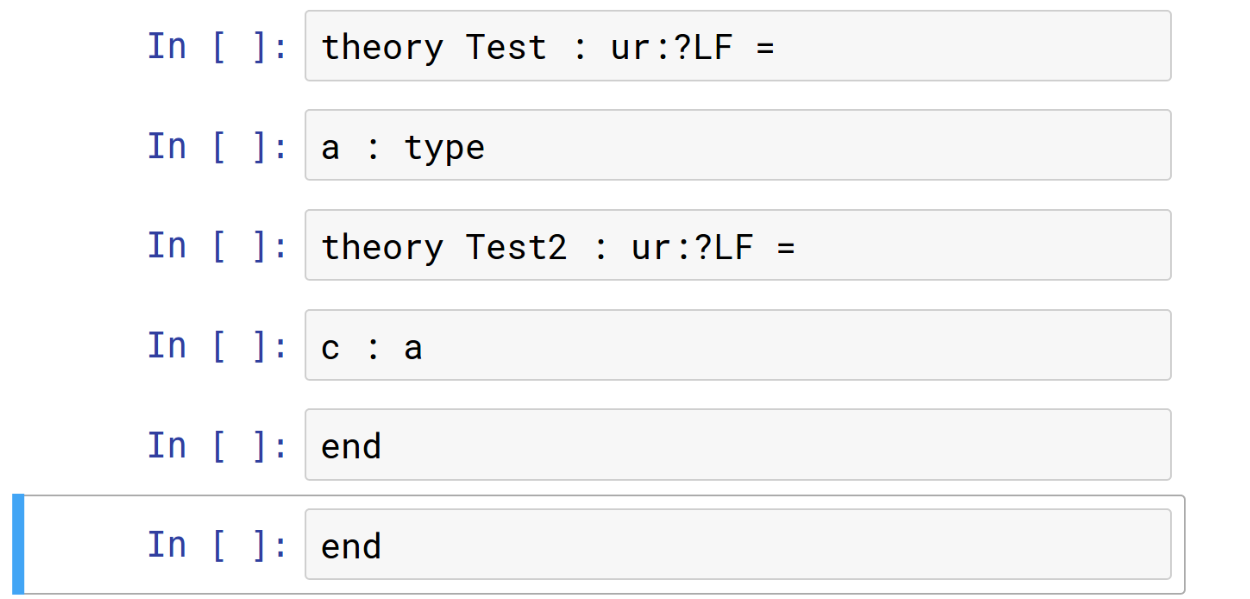
\includegraphics[width=10cm]{test_theory_jupyter}\end{minipage}
\begin{minipage}[c]{5cm}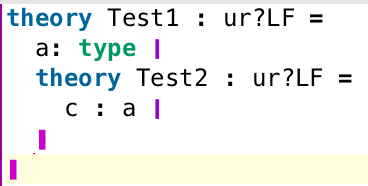
\includegraphics[width=5cm]{test_theory}\end{minipage}
\caption{Content Commands for Building Theory Graphs}\label{fig:test_theory}
\end{figure}

A special write-command is \texttt{eval T}.
It interprets \texttt{T} in the current scope, infers its type \texttt{A}, computes its value \texttt{V}, and then adds the declaration \texttt{resI:A=V} to the current theory, where \texttt{I} is a running counter of unnamed declarations.
This corresponds most closely to the REPL functionality in typical Jupyter kernels.

While write-commands correspond closely to the available types of MMT declarations, the set of read-commands is extensible.
For example, the commands \texttt{get U} where \texttt{U} is any MMT URI returns the MMT declaration of that URI.

\paragraph{Output}
The kernel returns the following kinds of return messages:
\begin{itemize}
\item \textbf{Admin messages} are strings returned in response to session management commands.
\item \textbf{New-element messages} return the declaration that was added by a write-command.
\item \textbf{Existing-element messages} return the declaration that was retrieved by a \texttt{get} command.
\end{itemize}
Like read-commands, the set of output messages is extensible.

The new-element and existing-element messages initially return the declaration in MMT's abstract syntax.
And a post-processing layer specific to Jupyter renders them in HTML+presentation MathML.
That way, the core kernel functionality can be reused easily in other frontends than Jupyter.

\subsection{Implementation}\label{sec:kernel:impl}

\paragraph{Overview}
Generally, Jupyter emphasizes protocols that specify the communication between frontend (i.e., usually Jupyter notebooks) and backend (i.e., kernels implemented in various programming languages).
This requires a certain duplication of implementation and, critically, maintenance, e.g., when implementing xeus, xwidgets and similar libraries for C++.
But the Python infrastructure for kernels is by far the best developed one, especially when it comes to Jupyter widgets. 
Therefore, it makes sense to implement our kernel on top of Python.
However, actually executing the user's commands requires a strong integration with the MMT implementation, which uses Scala.
That made it advisable to implement all Jupyter-specific functionality, especially the communication and management, in Python, while all mathematically relevant logic is handled in Scala.

Therefore, our implementation consists of three layers.
The top layer is a Python module that implements the abstract class for Jupyter kernels.
The bottom layer is a Scala class adding a general-purpose REPL to MMT that handles all the logic of MMT documents.
This can be reused easily in other frontends.
User commands are entered on the client and sent to the top layer, which forwards all requests to the bottom layer and all responses from the bottom layer to the client.
The communication between top and bottom layer is handled by a middle layer.
Its main purpose is to bridge between Python and MMT, format results in HTML, and add interactive functionality via widgets.

This bridging of programming languages is a generally difficult problem.
After some experiments with different solutions (e.g., HTTP communication) and discussion within the OpenDreamKit community, we identified the Py4J library~\cite{Py4J:on} as the best choice.
This is a Python-JVM bridge that allows seamless interaction between Python and any language (such as Scala) that compiles to the JVM.
Thus, our Python kernel can call MMT code directly.
Valuable Py4j features include callbacks from MMT to Python, shared memory (by treating pointers to JVM objects as Python values), and synchronized garbage collection.
That makes our kernel very robust against bit rot and allows benefiting from future improvements to the MMT backend.

Py4J is only JVM-specific, not Scala-specific.
That means that some Scala-specific constructs are not readily exposed to Python.
For example, both Python and Scala allow magic methods for treating any object as a function, but the JVM does not; moreover, the magic method is called \texttt{\_\_call\_\_} in Python and \texttt{apply} in Scala.
Similarly, Scala collections like lists are not automatically seen as their counterparts in Python.
Therefore, we wrote a Python module (which is distributed with MMT\footnote{This is currently at \url{https://github.com/UniFormal/MMT/blob/devel/src/python-mmt/example/mmt.py} but may be moved in the future.}) that performs the bureaucracy of matching up advanced Python and Scala features.


\subsection{Graphical User Interfaces via Jupyter Widgets}\label{sec:kernel:widgets}

Jupyter widgets are interactive GUI components (e.g., input fields, sliders, etc.) that allow Jupyter kernels to provide graphical interfaces.
While the concept is general, it is most commonly used to refer to the Python-based widget library developed for the Python kernel.
A widget encapsulates state that is maintained in an instance of a Python class on the server and displayed via a corresponding Javascript/HTML component on the client.
A major advantage of our kernel design is that we can reuse these widgets (via the to layer).

As our kernel's intelligence is maintained is maintained in MMT and thus Scala, we had to write some middle layer code to allow our kernel to create widgets.
This code uses Py4J to expose the widget-management functionality of the top layer to the lower layers.
This is done via a class of callback functions $C$ that are passed along when the former calls the latter.

\begin{figure}[ht]\centering
  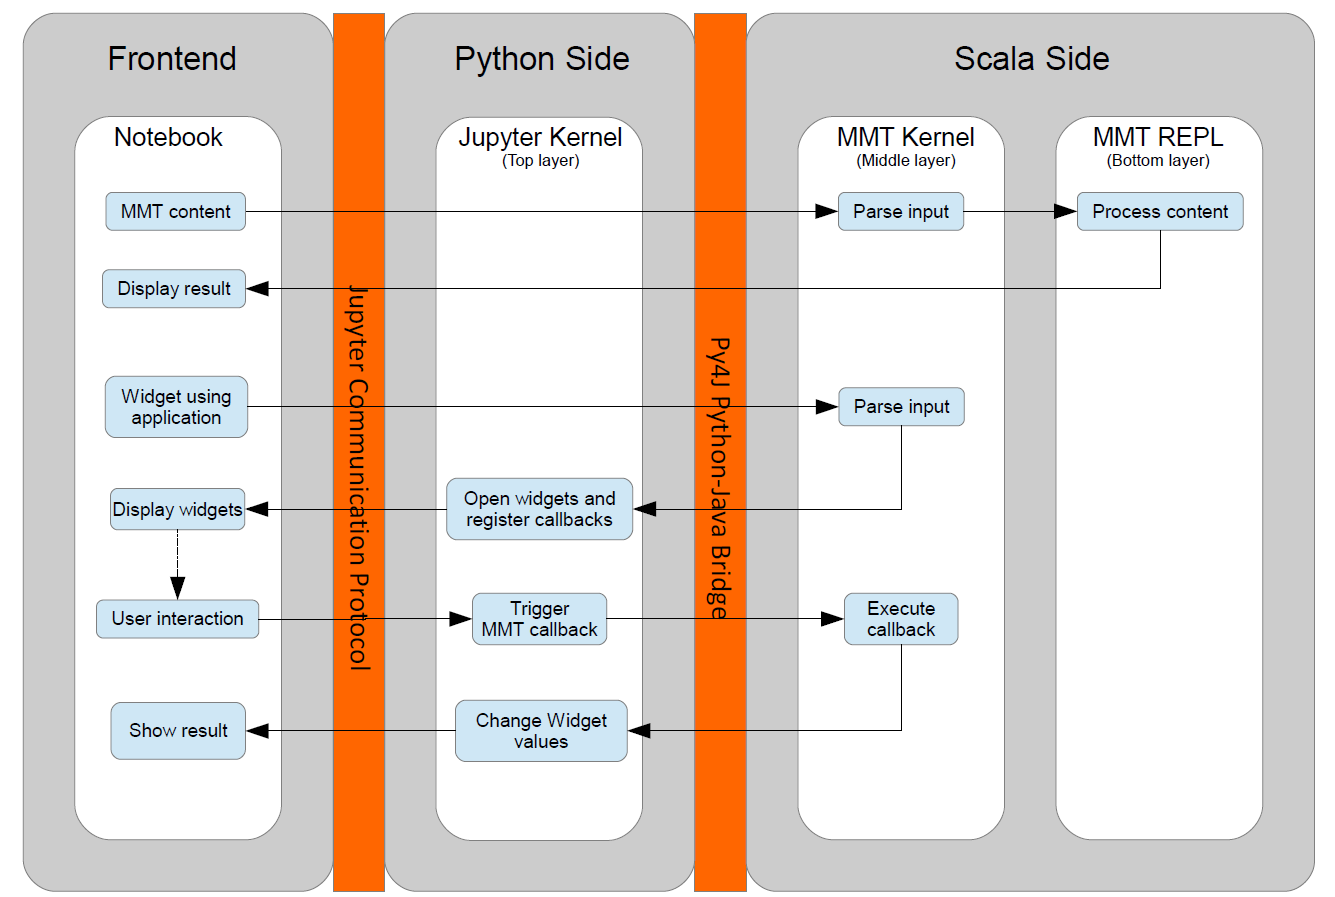
\includegraphics[width=12cm]{ArchitectureDiagram}
  \caption{Architecture diagram}\label{fig:architecture-diagram}
\end{figure}

Figure~\ref{fig:architecture-diagram} shows the details of the communication.
The upper part shows the simplest (widget-less) case: MMT content is entered in the frontend and forwarded to the bottom layer, and the response is forwarded in the opposite direction. (Steps that simply forward data from one layer to the next are not shown explicitly.)

The lower part shows a more complex widget-based interaction.
First of all, we add special management commands that are not passed on to the GUI-agnostic bottom layer.
Instead, they are identified by the middle layer, which responds by delegating to a GUI application.
This application then builds its graphical interface by calling the callbacks passed along by the top layer.
This results in a widget object in Python that is returned to the top layer and then forwarded to the frontend.

As usual, GUI components may themselves carry callback functions for handling events that are triggered by user interaction with the GUI in the frontend.
While conceptually straightforward, this leads to an unusually deep nesting of cross-programming language callbacks.
When creating a widget, the Scala-based GUI application may pass Scala callbacks $D$ whose implementation makes use of the $C$-callbacks provided by the top layer.
Thus, a user interaction triggers an MMT callback $D$ in the Python top layer, which is executed on the Scala side via Py4J, which in turn may call the Python callbacks $C$ exposed via Py4J.

Our design makes it very easy to build and deploy simple GUI applications for MMT --- we still have the full power of Jupyter widgets at our fingertips.

%\paragraph{Jupyter/MMT Widgets}
%The use of a Python-JVM bridge pays off in particular when it allows us to reuse the widget library that is already part of the Python codebase of Jupyter.
%It allows the top layer to call the middle layer in a way that passes the Python-based kernel environment of the top layer.
%That way, the Scala-based middle layer can perform callbacks to the widget library.
%Thus, the middle layer can choose to present some of the messages returned by the bottom layer as interactive HTML using widgets.
%
%For example, when presenting a parametric theory as HTML+MathM, we can add a text input field next to every parameter.
%Whenever the strings in these fields change, the frontend notifies the top layer, which passes on the change to the middle layer.
%The middle layer then parses these strings and substitutes them in the body of the resulting declaration.
%This is similar to but more general than the typical Jupyter functionality of rerunning a notebook when an input cell changes: while Jupyter uses a list of input cells and any change affects all subsequent cells, our widget amounts to a tree structure in which input fields have local, nested scope.
%
%\ednote{@Kai: this is a simple application that we might not finish by the deliverable deadline but that you should implement nonetheless. Stay in touch with me on the details. KA: for this we would probably need a custom widget}

\paragraph*{Example: In-Document Computation}
We present a simple example of a GUI application for in-document computation as specified D4.9~\cite{ODK-D4.9}.
It is triggered by the special command \texttt{active computation} and builds a GUI consisting of a few standard Jupyter widgets: a label, a button (labeled \textit{compute}), three text input fields, and one button widget.
A concrete example can be seen in Figure~\ref{fig:ac}.
This shows a notebook in which our application is returned as the response to cell \texttt{In[1]}.


\begin{figure}[ht]\centering
  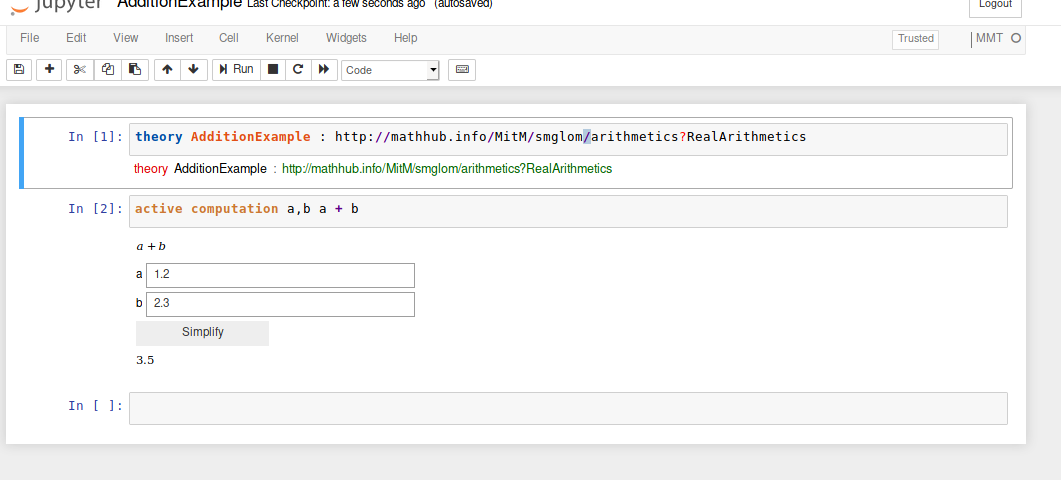
\includegraphics[width=12cm]{activecomp}
  \caption{Active Computation in Jupyter Notebooks via Jupyter/MMT Widgets}\label{fig:ac}
\end{figure}

The three text input fields contain values linked by an equation, in this case $E=mc^2$.
The user can edit these fields and press the button to compute the other values.
In that case, a the button carries the callback $D$, which results in a call to our application on the Scala side.
It uses MMT to perform the computation and then calls the $C$ callbacks to update the values in the widgets.
No additional work is needed to implement the synchronization between the Python top layer and the HTML frontend as this is a standard feature of Jupyter widgets.

%%% Local Variables:
%%% mode: latex
%%% mode: visual-line
%%% fill-column: 5000
%%% TeX-master: "report"
%%% End:

%  LocalWords:  Jupyter newpart textbf ednote centering texttt includegraphics synchronized customizable inparaenum Realizing subsubsection


\section{Jupyter Notebooks in MathHub}\label{sec:nb-mh}
We present the integration of Jupyter Notebooks into the MathHub system.

\ednote{TW: Update this with the actual MH Structure}

\subsection{Overview}

\begin{newpart}{FR@TW: check if true}
Our system consists of four components:
\begin{compactitem}
\item A GitLab repository hosting server\footnote{\url{http://gl.mathhub.info}} provides persistent storage of documents in any format, including their OMDoc representation.
\item An MMT instance\footnote{\url{http://mmt.mathhub.info}} uses the OMDoc representations to provides the shared knowledge space and provides a high-level API for it.
\item A Jupyter Notebook server\footnote{\url{http://jupyter.mathhub.info}} provides web-based IDE for editing interactive documents.
\item The MathHub frontend\footnote{\url{http://mathhub.info}} serves as the main entry point and delegates some subtasks to the former.
\end{compactitem}

The Jupyter server is an out of the box installation of Jupyter except for additionally supporting our new MMT kernel.
\ednote{Update URL strucure}
Consequently, the integration between the Jupyter and the MathHub frontends is shallow: MathHub opens Jupyter Notebooks in separate tabs or iframes using URLs served by Jupyter.
We would have preferred to deeply integrate the Jupyter frontend into MathHub, e.g., by using Jupyter simply as a JavaScript library in MathHub.
But that is infeasible because Jupyter is primarily used as a monolithic system not designed to allow deep integration.\footnote{The most recent versions of Jupyter are aiming to allow it, but at present any deep integration would realistically be too brittle to be worthwhile.}
\end{newpart}

\subsection{Notebooks as Standalone Documents}

The MathHub frontend already provides special interaction functionality for individual document types.
We used this by making Jupyter Notebooks a new document type; see Figure~\ref{fig:mathhub-NB} for an example.
When displaying a known document type, the frontend shows multiple tabs.
For Notebooks, these are the following:
\begin{compactenum}[\em i\rm)]
\item \textsf{view} gives a preview of the notebook, essentially the computation cells without output, pre-rendered for static serving without involving Jupyter at all.%
\ednote{MK: we should implement this; I am not sure what the best way is for this. I guess a build target based on \texttt{https://github.com/jendas1/jupyter-notebook-quick-look}.}
\item \textsf{run/edit} opens the respective notebook on the Jupyter server for execution and editing.
Any changes to the Notebook made from within Jupyter can be committed back to the Git repository. 
\item \textsf{metadata} (this is the tab open in Figure~\ref{fig:mathhub-NB}), shows the metadata provided by the Jupyter kernel and the repository. 
\item \textsf{source} provides access to the document source; here simply a link to the notebook file in the Git repository.
\item \textsf{statistics} shows statistical information about the notebook, its corresponding MMT document, and its connections with other MMT documents in the background knowledge base.
\item \textsf{graph} links to graph-based visualizations of the document including the theory graph, declaration graph, and dependency graph, using our TGView system, a canvas-based in-browser visualizer for knowledge graph information~\cite{RupKohMue:fitgv17}.
\end{compactenum}
This integration combines the interactive features of the Jupyter server with the knowledge management facilities on MathHub. In the future, we plan to integrate the notebook diff/patch \textsf{nbdime} developed in OpenDreamKit to extend the knowledge management facilities. 

\begin{figure}[ht]\centering
  \fbox{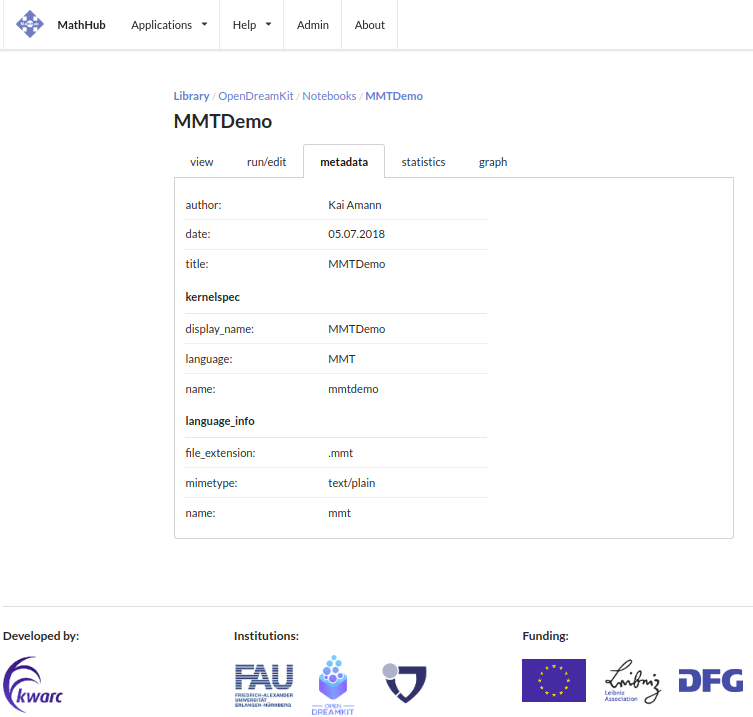
\includegraphics[width=13cm]{../D4.11/NB-Mathhub}}
  \caption{A Jupyter Notebook in MathHub (Metadata)}\label{fig:mathhub-NB}
\end{figure}
\ednote{TW: Wait, this exists?}
%A Jupyter Notebook additionally has a special button appears that allows users to open the notebook in the associated Jupyter server. Currently these notebooks do not use the MMT process running on MathHub.info, due to the architecture of the MMT Kernel. Therefore they currently do not have access to the MathHub universe. \ednote{KA: if the Kernel server would run on the same VM as the MathHub MMT we could give the kernel access to it}
%\ednote{@Kai, @Tom: check this, do the implementation}

\ednote{@KA: write the example from Fig.~\ref{fig:test_theory} as a Jupyter notebook, store the file somewhere on gl.mathhub.info and give a link to the Fig.~\ref{fig:mathhub-NB} view of that notebook}

\subsection{Notebooks as Parts of Static Documents}

To interact dynamically with content in arbitrary MathHub documents, we added a new feature that creates a new ephemeral Jupyter Notebook and inserts it (via an iframe) into the current document.
Importantly, the new Notebook is prefilled with an import of the current context so that users can Here we can feed the document context information into the interior notebook.

\begin{figure}[ht]\centering
  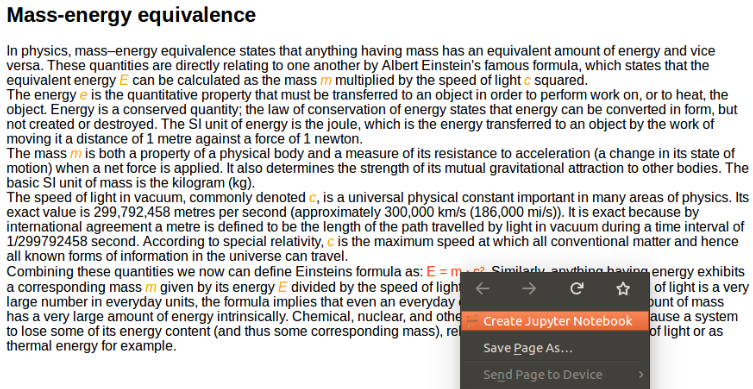
\includegraphics[width=15cm]{../D4.11/conversionHTML}
  \caption{HTML document and the context menu for converting}\label{fig:conversionHTML}
\end{figure}
\ednote{Re-do this screenshot cleanly}

Continuing the example from the previous section, Figure~\ref{fig:conversionHTML} shows a scientific HTML document that contains the equation $E=mc^2$.
\ednote{MK@KA/FR: We should make an sTeX document that contains $E=mc^2$ (e.g. by copying parts of \texttt{https://en.wikipedia.org/wiki/Mass-energy\_equivalence}) and really implement the in-document computation example.}
The user can use the context menu to trigger the notebook generation on this formula.
The context menu is generated using JavaScript that picks up on annotations of formulas with specific CSS classes.
Currently the author has to manually annotate the formulas, but we are working on a mechanism to automatically create it from the document context.

\ednote{Describe structure of tags within the HTML}
Figure~\ref{fig:conversionNotebook} shows the notebook created by our tool.
Note that the generated notebook starts with several \texttt{include} declarations that import the context of the formula.
These are generated by MathHub to obtain a minimal standalone MMT theory in which the respective formula is well-formed. 

If desired, the notebooks can be easily uploaded to the Jupyter server, stored persistently in the repository server, or evaluated in a locally deployed version of the system per drag-and-drop.

%The two predominant cell types in Jupyter notebooks are \texttt{code} and \texttt{markdown} cells. 
%Code Cells contain user input, like described in section \ref{sec:kernel:syntax}.
%The HTML elements that contain the input for these code cells are usually not visible, since they do not fit into the context of a scientific document and may not be understood by reviewers that are not familiar with MMT syntax. 
%The other cell type: markdown cells, can contain any type of plain text and support GitHub flavoured markdown. 
%Therefore markdown cells are used for providing notebooks with additional selectable information from the original HTML document.

\begin{figure}[ht]\centering
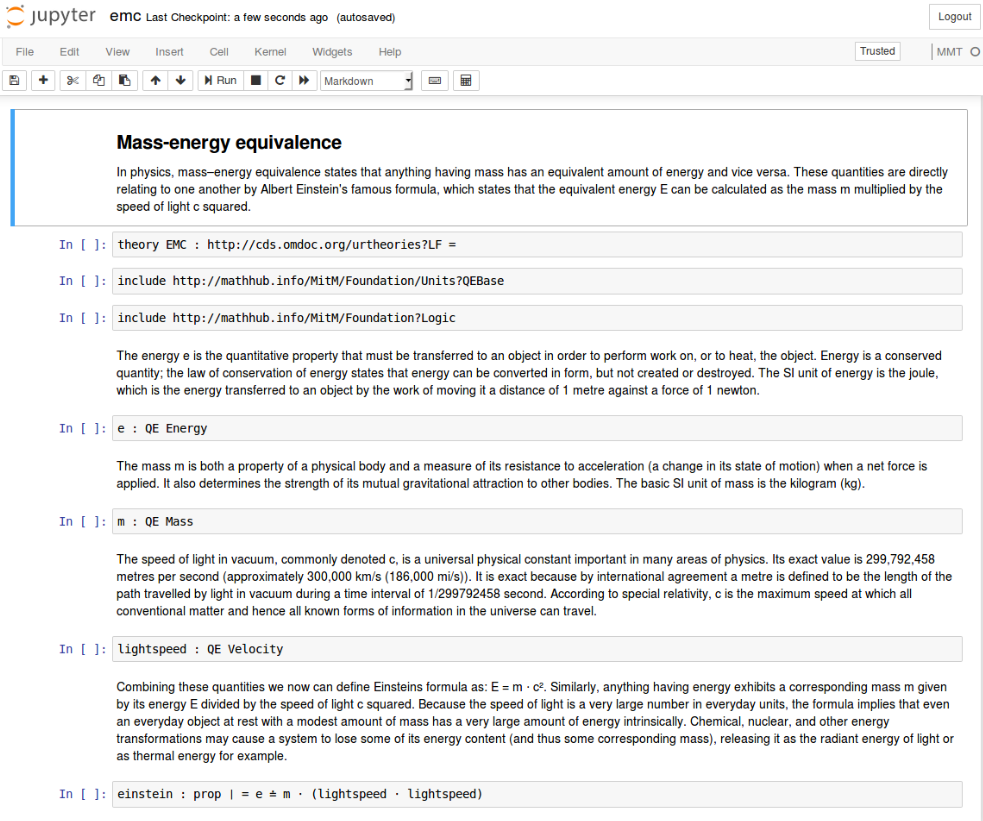
\includegraphics[width=15cm]{../D4.11/conversionNotebook}
\caption{The resulting Jupyter notebook}
\label{fig:conversionNotebook}
\end{figure}
\ednote{run all cells}

%%% Local Variables:
%%% mode: latex
%%% mode: visual-line
%%% fill-column: 5000
%%% TeX-master: "paper"
%%% End:

%  LocalWords:  Jupyter ednote compactenum textsf texttt visualizations RupKohMue:fitgv17 nbdime centering fbox includegraphics NB-Mathhub


\section{Applications}\label{sec:mitm-nb}
  The immediate application of the Jupyter/MMT integration presented in this paper is interacting with MMT in a REPL.
  The MMT tool ecosystem only really supported IDE-interaction with MMT libraries via JEdit and (recently) IntelliJ IDEA plugins. 
  While the MMT system provides a simple shell for interaction, this was only used for configuration and setup of the MMT process.
  We anticipate that the REPL-like interaction will feel more natural for users of interactive theorem provers and computer algebra systems.
  Even for the new MathScheme-style of specifying theory graph libraries via theory combinators~\cite{ShaRab:dcm19} e.g.,
\begin{lstlisting}[mathescape]
semigroup = extend magma by {assoc: $\vdash\forall{a,b,c}:G. a\circ (b\circ c) = (a\circ b)\circ c $}
\end{lstlisting}
  is well-suited to development/experimentation in a REPL followed by generating an OMDoc file from the recorded notebook.

\subsection{Towards a Virtual Research Environment based on the Math-in-the-Middle Paradigm}


Another direct application is in the context of the OpenDreamKit project, which integrates various independently developed computational engines into a mathematical virtual research environment following the Math-in-the-Middle (MitM) approach~\cite{DehKohKon:iop16}.
This uses the MMT language for formalizing mathematical background knowledge (which we store in MathHub documents of type MMT) and the MMT system for integrating computation tools.
Therefore, Jupyter-MMT notebooks can serve as a unified user interface for MitM systems.

For example, consider the theory\footnote{Available at \url{https://gl.mathhub.info/ODK/lmfdb/blob/master/source/schemas/tutorial_example.mmt}}  in Figure~\ref{fig:hecke}, which serves as our standard example for the interaction between MMT and LMFDB (a large database of mathematical objects that was integrated with MMT in previous deliverables of OpenDreamKit).
We can now rewrite it as a notebook.

A screenshot of the resulting notebook, as displayed by a Jupyter server running our MMT kernel, is shown in Figure~\ref{fig:lmfdbexample}.

\begin{wrapfigure}{r}{0.7\textwidth}
  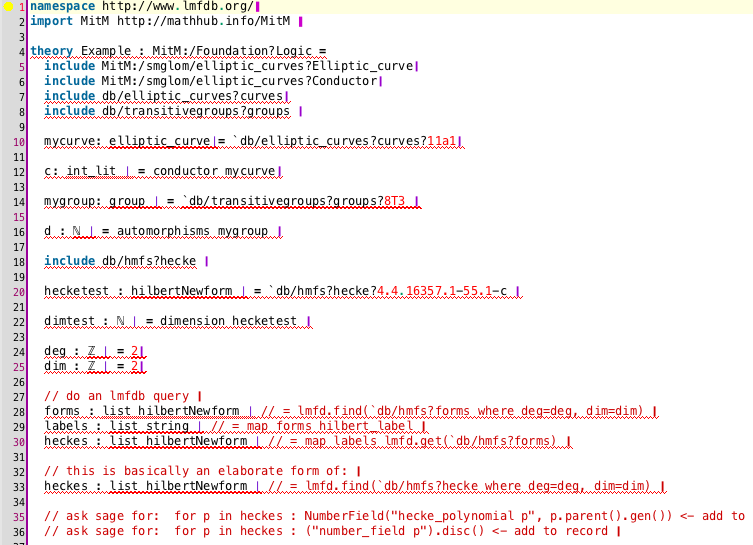
\includegraphics[width=\linewidth]{../D4.11/hecke}\vspace*{-1em}
  \caption{A Theory for LMFDB/MMT Interaction}\label{fig:hecke}\vspace*{-3em}
\end{wrapfigure}
The selected declaration of \texttt{mycurve} accesses the elliptic curve \texttt{11a1} that is stored in LMFDB.
When the Jupyter kernel for MMT processes this command, the bottom layer of the kernel dynamically retrieves this curve from LMFDB and builds from it an object of type \texttt{elliptic\_curve} in the MitM ontology.\bigskip

\begin{figure}[ht]\centering
  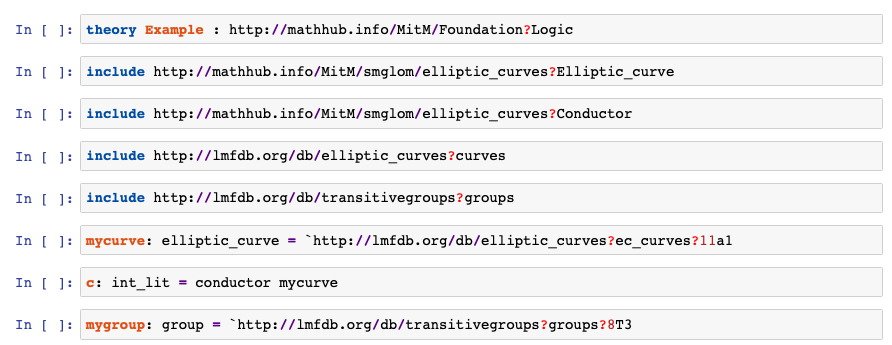
\includegraphics[width=0.9\textwidth]{screenshots/heckenb}
  \caption{The Beginning of the Notebook for the theory from Figure~\ref{fig:hecke}}\label{fig:lmfdbexample}
\end{figure}

\subsection{Domain specific applications e.g., MoSIS}
Our second case study addresses a \emph{knowledge gap} that is commonly encountered in computational science and engineering:
To set up a simulation, we need to combine domain knowledge (usually in terms of physical principles), model knowledge (e.g., about suitable partial differential equations) with simulation (i.e., numerics/computing) knowledge.
In current practice, this is resolved by intense collaboration between experts, which incurs non-trivial translation and communication overheads.
With the infrastructure presented in this paper, we can do better.
In fact, the MoSIS application was developed in parallel to our Jupyter/MathHub integration and MoSIS requirements helped inform the the development.
We have ported the original version~\cite{PolKohKoe:kacse18} to the new infrastructure, simplifying and extending it in the course.
All in all, the interaction part of the MoSIS project would now be a straightforward software development exercise instead of a contribution of its own. 

\begin{figure}[ht]\centering
  \begin{minipage}[c]{.49\textwidth}
    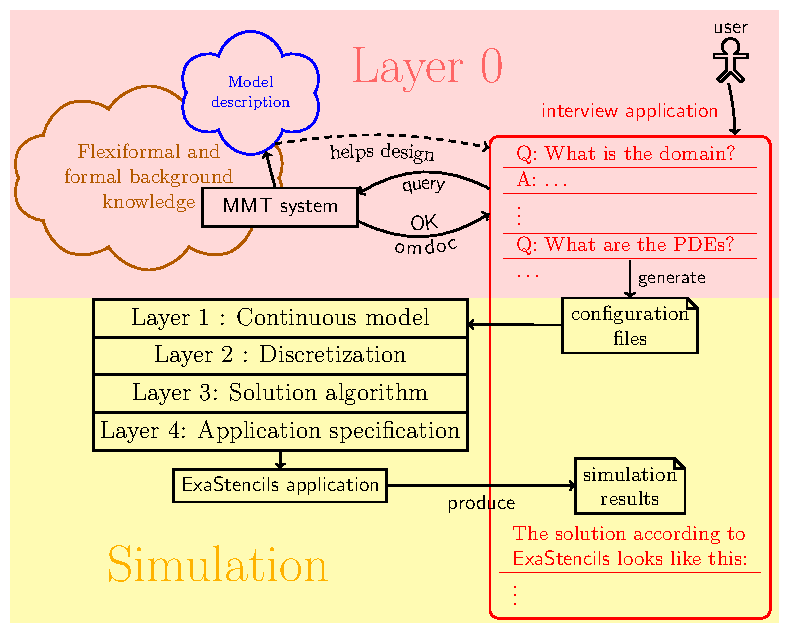
\includegraphics[width=\textwidth]{../D4.11/proto}
  \end{minipage}
  \begin{minipage}[c]{.49\textwidth}
    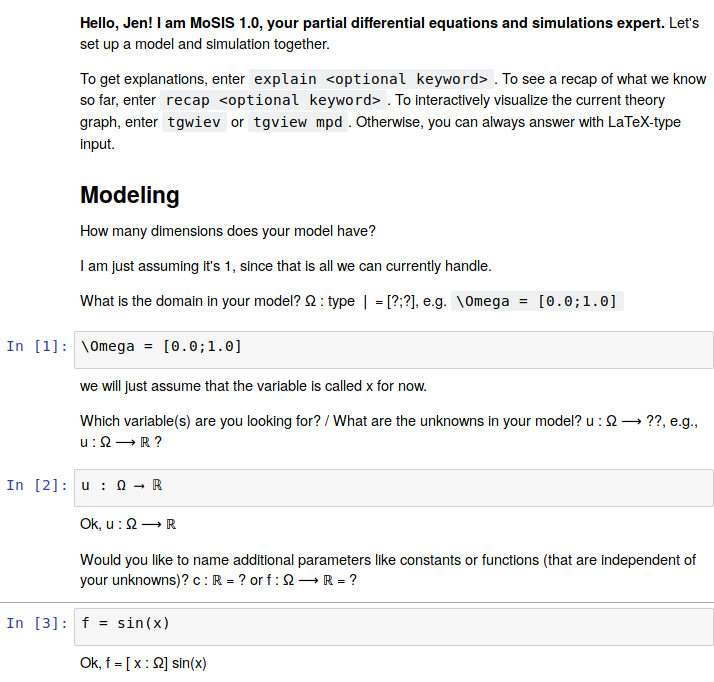
\includegraphics[width=\textwidth]{../D4.11/Screenshot_interview}
  \end{minipage}
  \caption{MoSIS Information Architecture and Dialogue}\label{fig:prototype}
\end{figure}

Concretely, MoSIS uses a Jupyter notebook that has access to an MMT theory graph on MathHub.info.  Our Jupyter/MMT/MathHub integration enabled building an interview application that hides these mathematical details from the user.

Based on this theory graph, we built a targeted knowledge acquisition dialog that supports the formalization of domain knowledge, combines it with simulation knowledge and finally drives a simulation run --- all integrated into a Jupyter Notebook.
Figure~\ref{fig:prototype} shows the general architecture:
The left side shows the simulation engine \textsf{ExaStencils}~\cite{exastencils.on} and the MMT system that acts as the theory graph interface.
The right hand side shows the interview --- a Jupyter notebook --- as the active document and how it interacts with the MMT kernel.
The user only sees the notebook.
She answers the knowledge acquisition questions presented by MoSIS until MoSIS can generate a configuration file for ExaStencils.
The latter builds efficient code from it through the ExaSlang layers and computes the results and visualizations, which MoSIS in turn incorporates into the notebook. 

%%% Local Variables:
%%% mode: latex
%%% mode: visual-line
%%% fill-column: 5000
%%% TeX-master: "paper"
%%% End:

%  LocalWords:  MitM-Based Formalized formalizing Jupyter-MMT ednote summarize centering includegraphics textwidth Jupyter fig:lmfdbexample texttt mycurve texttt textbf lmfdb_example emph PolKohKoe:kacse18 fig:pde-theory fbox textheight pde-theory formalization textsf exastencils.on visualizations newpart JEdit DehKohKon:iop16 ShaRab:dcm19 wrapfigure vspace bigskip heckenb Mathhub


\section{Conclusion and Future Work}\label{sec:concl}
\section{Conclusion}\label{sec:concl}

We have shown how to extend the Math-in-the-Middle framework for integrating systems to mathematical data bases like the \lmfdb. 
The main idea is to embed knowledge sources as virtual theories, i.e. theories that are not -- theoretically or in practice -- limited in the number of declarations and allow dynamic loading and processing. 
For accessing real-world knowledge sources, we have developed the notion of codecs and integrated them into the MitM ontology framework. 
These codec's (and their MitM types) lift knowledge source access to the MitM level and thus enable object-level interoperability and allow humans (mathematicians) access using the concepts they are familiar with. 
Finally, we have shown a prototypical query translation facility that allows to delegate some of the processing to the underlying knowledge source and thus avoid thrashing of virtual theories. 

\paragraph{Related Work} Most other integration schemes employ a \textbf{homogenous approach}, where there is a master sytsem and all data is converted into that system. 
A paradigmatic example of this is the Wolfram Language and the Wolfram Alpha search engine~\cite{WolframAlpha:on}, which are based on the Mathematica kernel. 
This is very flexible for anyone owning a Matheamtica license and experienced in the Mathematica language and environment.

The MitM-based approach to interoperability of data sources and systems proposed in this paper is inherently a \textbf{heterogeneous approach}: systems and data sources are kept ``as is'', but their APIs are documented in a machine-actionable way that can be utilized for remote procedure calls, content format mediation, and service discovery. 
As a consequence, interaction between systems is very flexible.
For the data source integration via virtual theories presented in this paper this is important. 
For instance, we can just make an extension of \mmt or Sage which just act as a programmatic interface for e.g. \lmfdb. 

\paragraph{Future Work}
We have discussed the MitM+virtual theories methodology on the elliptic curves sub-base of the \lmfdb, which we have fully integrated. 
We are currently working on additional \lmfdb sub-bases. 
The main problem to be solved is to elicit the information for the respective schema theories from the \lmfdb community. 
Once that is accomplished, specifying them in the format discussed in this paper and writing the respective codecs is straightforward. 

Moreover, we are working on integrating the the Online Encyclopedia of Integer Sequences (OEIS~\cite{Sloane:OEIS,oeis}). 
Here we have a different problem: the OEIS database is essentially a flat ASCII file with different slots (for initial segments of the sequences, references, comments, and formulae); all minimally marked up ASCII art. 
In~\cite{LuzKoh:fsarfo16} we have already (heuristically) flexiformalized OEIS contents in \ommt; the next step will be to come up with codecs based on this basis and develop schema theories for OEIS.

\subsubsection*{Acknowledgements}
The authors gratefully acknowledge the fruitful discussions with other participants of
work package WP6, in particular John Cremona on the LMFDB and Dennis M\"uller on early
versions of the \ommt-based integration. We acknowledge financial support from the
OpenDreamKit Horizon 2020 European Research Infrastructures project (\#676541).

%%% Local Variables:
%%% mode: latex
%%% TeX-master: "paper"
%%% End:

%  LocalWords:  sec:concl subsubsection ommt lmfdb itemize Sloane:OEIS,oeis LuzKoh:fsarfo16 flexiformalized MitM-based textbf utilized


\printbibliography

\end{document}

%%% Local Variables:
%%% mode: latex
%%% mode: visual-line
%%% fill-column: 5000
%%% TeX-master: t
%%% End:

%  LocalWords:  maketitle newpage tableofcontents newpage newcommand xspace ednote mathdb flexiformal inparaenum environmnet setcounter tocdepth sec:nb-mh appl
%  LocalWords:  standardize dktheories concl printbibliography pn textit mmt mitm emph
%  LocalWords:  WPref dksbases prioritized taskref organized delivref dkstheories Jupyter
%  LocalWords:  githubissuedescription JEdit visualization subsubsection Py4JGateway
%  LocalWords:  Runme formalization oldpart PolKohKoe:kacse18a

